\documentclass[12pt,a4paper]{article}
\usepackage[utf8]{inputenc}
\usepackage[danish]{babel}
\usepackage{amsmath}
\usepackage{amsfonts}
\usepackage{amssymb}
\usepackage{graphicx}
\usepackage[left=2cm,right=2cm,top=2cm,bottom=2cm]{geometry}


\usepackage{titlepic}
\usepackage{enumerate}
\usepackage{enumitem}
\usepackage{float}
\usepackage{pdfpages}
\usepackage[colorlinks = true,
            linkcolor = blue,
            urlcolor  = blue,
            citecolor = blue,
            anchorcolor = blue]{hyperref}
\usepackage[explicit]{titlesec}
\usepackage{pstricks}
\usepackage[amsmath,thmmarks]{ntheorem} %pakke til at lave sætningsenvorinmets (kan ikke loades sammen med amsthm)
\usepackage{color}
\usepackage{tikz}

%opretter environmets til sætningsstrukturen 
\theorembodyfont{\normalfont}

	
	%sætnings environment	
	\newtheorem{thm}{Sætning}

	\theoremstyle{break}	
	%opgave environment	
	\newtheorem{opg}{Opgave}	

	%Korrolar environment
	\newtheorem{korollar}[thm]{Korollar}	
	
	%Lemma environment	
	\newtheorem{lemma}[thm]{Lemma}
	
	\theoremsymbol{\ensuremath{\circ}}	
	
	%definition environment	
	\newtheorem{definition}[thm]{Definition}
	
	%eksempel environment	
	\newtheorem{eksempel}[thm]{Eksempel}
	
	
	
	%Bevis environment
	\theoremstyle{nonumberplain}
	\theoremheaderfont{%
	\normalfont\itshape}
	\theorembodyfont{\normalfont}
	\theoremsymbol{\ensuremath{\square}}
	\theoremseparator{.}
	
	\newtheorem{proof}{Bevis}
	\newtheorem{los}{Løsning}
	






\setlength\parindent{0pt}

%\titleformat{\section}{\Large\bfseries}{}{0pt}{#1}
%\titleformat{\subsection}{\large\bfseries}{}{0pt}{#1}


%nye komandoer
\newcommand{\mR}{\mathbb{R}}
\newcommand{\mZ}{\mathbb{Z}}
\newcommand{\mN}{\mathbb{N}}
\newcommand{\mQ}{\mathbb{Q}}
\newcommand{\mC}{\mathbb{C}}
\newcommand{\hs}{\hspace{2mm}}
\newcommand{\Hs}{\hspace{4mm}}
\newcommand{\pipe}{\hs | \hs}
\newcommand{\lp}{\left(}
\newcommand{\rp}{\right)}
\newcommand{\vect}[1]{\underline{#1}}
\newcommand{\matr}[1]{\underline{\underline{#1}}}
\newcommand{\cnum}[1]{\raisebox{.5pt}{\textcircled{\raisebox{-.9pt} {#1}}}}




\author{Mikkel B. Goldschmidt \\ Fysik A - Nørre Gymnasium}
\title{Rapport - Papirkuglekanon}
\date{\today}



\begin{document}
\maketitle

\section{Formål}
Jeg vil i denne rapport beskrive en elastikkanon vi har bygget. 
Vi forsøgte at skyde en papirkugle 4 meter ind i en cirkel med en halv meters diameter.
Jeg vil forsøge at beskrive relevante fysiske sammenhænge, der kan forklare hvordan kanonen kunne bygges til at skyde præcist. 
Til sidst vil jeg forsøge at forklare hvorfor det ikke lykkedes os at ramme cirklen.

\section{Teori}
Vores opstilling kan betragtes som en bevægelse i to dimensioner.
Jeg vil forsøge at beskrive denne bevægelse ved at betragte de forskellige kræfter der påvirker forsøget.
Derudover vil jeg forsøge at beskrive en metode til at finde ud af hvor kraftigt elastikkanonen skyder, da dette er helt essentielt for at ramme præcist.

\subsection{Beskrivelse af bevægelsen}
Under bevægelsen er der kun en kraft der påvirker papirkuglen nemlig tyngdekraften.
Derudover er der så en fart som kuglen er blevet skudt afsted med.
Denne fart vil jeg vise en måde at beregne på i næste afsnit, men i dette afsnit vil jeg blot betegne den som $v_s$.
Da bevægelsen forgår i to dimensioner, vil det gør beregningerne nemmere at betragte bevægelsen opdelt vandret og lodret.
For nemmere notation vil jeg lægge et koordinatsystem ind over mit forsøg og betragte lodret som $y$ og vandret som $x$, hvor $(0,0)$ ligger ved jorden under der hvor papirkuglen skydes afsted fra.

Jeg vil nu forsøge at beskrive startfarten i henholdsvis $x$
- og $y$-retningen udfra startfarten og vinklen der skydes afsted fra i forhold til lodret - kald denne vinkel $\theta$.
Det ses forholdvist nemt ved at tegne det som kraftpile at $v_x = cos(\theta )v_s$ og $v_y = sin(\theta )v_s$.

Da der ikke er nogle kræfter der påvirker kuglen i x-retningen, kan vi lave en stedfunktion i x-retningen i forhold til tiden: $$x(t) = v_x t$$

I y-retningen skal vi så også tage højde for tyngdeaccelerationen.
Dermed får vi en stedfunktion på formen (ses fra generel stedfunktion i en dimension): $$y(t)=-\frac{1}{2}gt^2+v_yt+h$$
hvor $h$ beskriver den højde kuglen skydes afsted over jorden.
\begin{figure}
\center
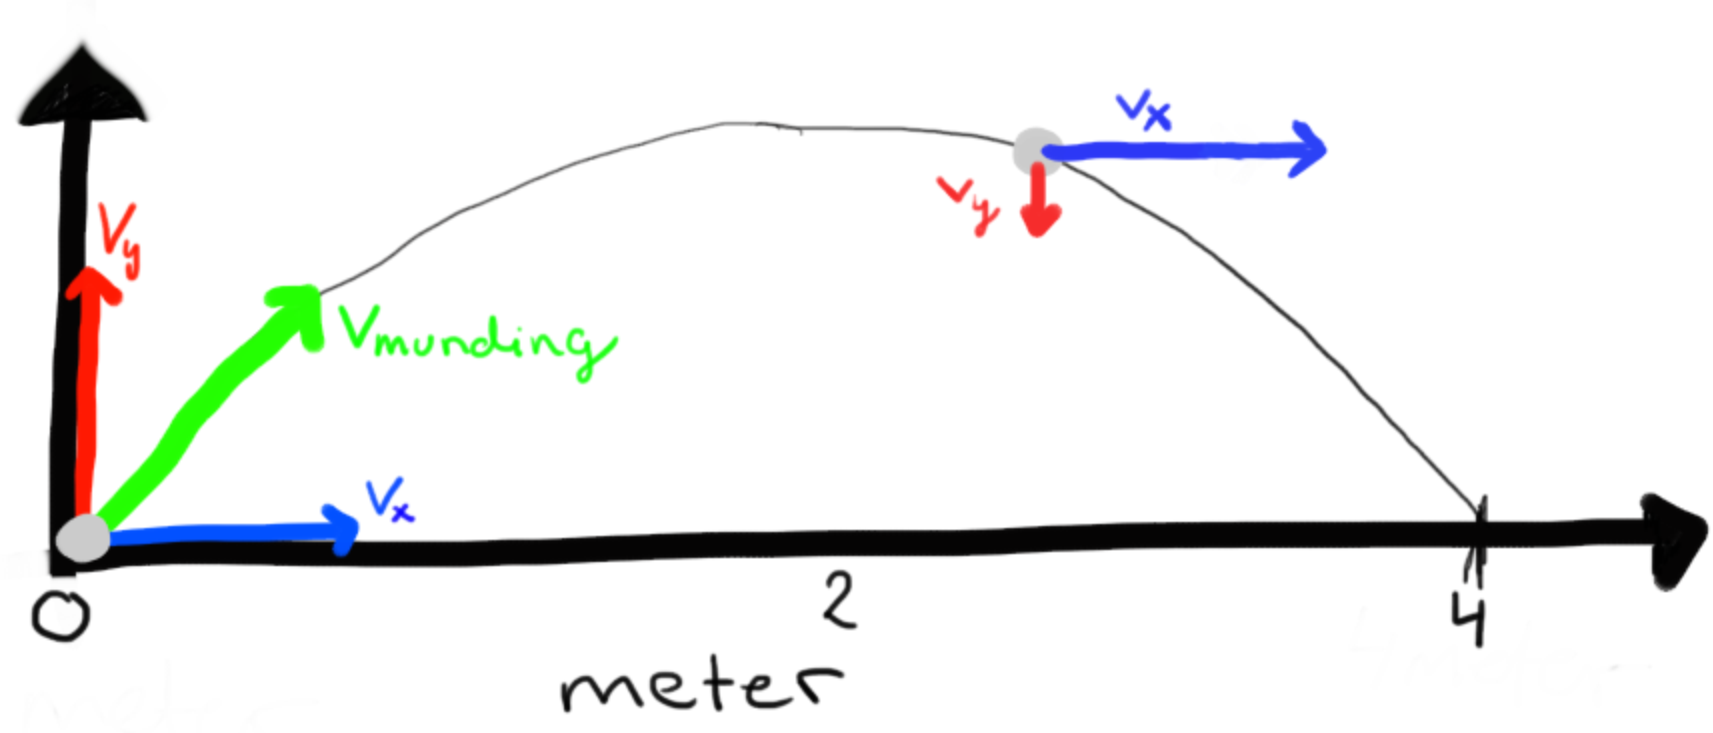
\includegraphics[scale=0.4]{diagram}
\caption{Indtegnede hastighedsvektorer ved bevægelsen. En indtegning ved affyring og en indtegning efter kuglener begyndt at falde. Bemærk at $v_x$ er uforandret mens $v_y$ ændres grundet tyngdekraften.}
\end{figure}

\subsubsection{Hvornår rammer kuglen jorden?}
Jeg vil nu forsøge at bestemme hvor langt fra udgangspunktet kuglen vil ramme ved brug af de to før udledte sammenhænge.

Jeg vil starte med at bestemme det tidspunkt $t_{slut}$ hvor kuglen vil ramme jorden.
Dette må være det positive tal $x$ der opfylder $y(x)=0$. 
Denne værdi kan findes forholdsvist nemt ved at løse for x som en andengradsligning:
$$t_{slut} = \dfrac{v_y + \sqrt{v_y^2 + 4 \cdot \frac{1}{2}gh}}{g}$$

Vi kan her udnytte at $v_y = sin(\theta )v_{munding}$ hvis vi er interesserede i at bestemme hvilken vinkel der skal skydes med for at opnå en bestemt afstand.

Når denne tid er bestemt, kan man nemt bestemme hvor langt fra udgangspunktet kuglen vil ramme ved at finde $x(t_{slut})$.

\subsection{Bestemmelse af mundingshastigheden}
For at beregne mundingshastigheden på vores papirkugleskydemaskine, kan man gør det at man skyder direkte op i luften fra nede fra gulvet og måle hvor lang tid det tager før kuglen rammer gulvet.
Da vil vi have en endimensional bevægelse med en enkelt kraft der påvirker kuglen (tyngdekraften). 
Vi må da kunne beskrive højde over jorden som en funktion $h$ af tiden:
$$h(t)=-\frac{1}{2}gt^2 + v_{munding}t$$
Da $t$ er en størrelse vi måler og $g$ er en kendt størrelse, vil vi nu kunne bestemme mundingshastigheden ved at finde en passende værdi for $v_{munding}$ så $h(t)=0$.
\pagebreak
\section{Forsøg}
Til forsøget byggede vi en kanon som den der kan ses på figur \ref{maskine}. 
Den fungerede ved at vi trak kuglen tilbage med en elastik og slap den løs så elastikken skød kuglen afsted. 
Ved at markere en længde elastikken skulle trækkes tilbage, kunne vi sikre at elastikken tilførte den samme mængde energi til kuglen hver gang vi skød. 

\begin{figure}
\center
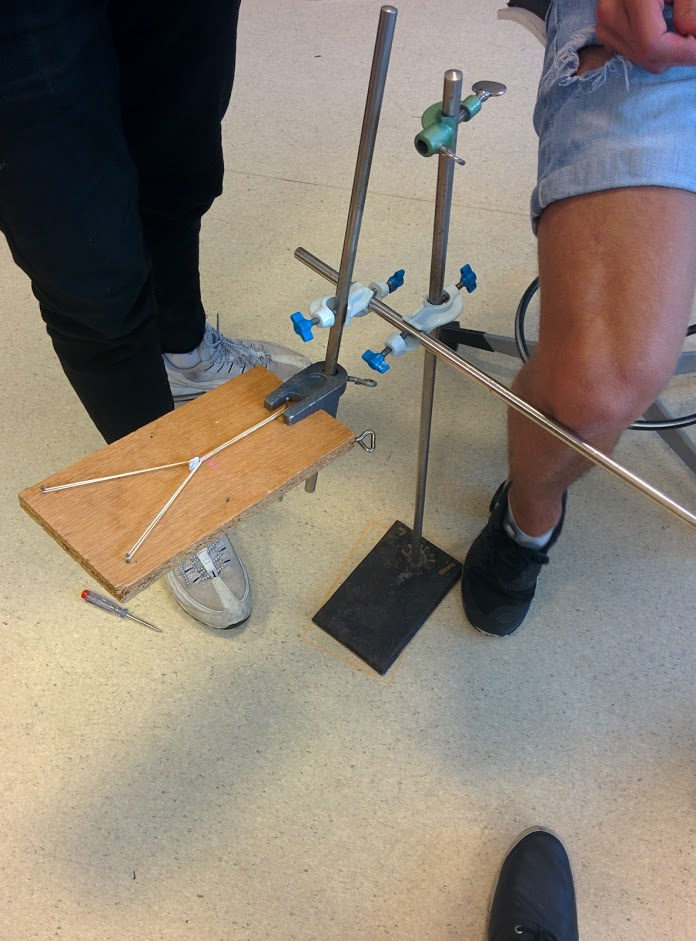
\includegraphics[scale=0.2]{papirkuglekastemaskine}
\caption{Vores papirkugleskydemaskine}
\label{maskine}
\end{figure}

\subsection{Bestemmelse af mundingshastighed}
Vi startede da med at bestemme mundingshastigheden. 
Da vi skød kuglen op lige op i luften fra det punkt vi havde valgt at trække elastikken til gik der ca. 1,3 sekunder før kuglen ramte jorden. 
Vi kunne da beregne en mundingshastighed ved at bruge sammenhængen der blev beskrevet i teoriafsnittet:
$$-\frac{1}{2}g(1.3s)^2 + v_{munding}(1.3 s)=0 \Rightarrow v_{munding}\approx6.4 \frac{m}{s}\approx 23 \frac{km}{t}$$

\subsection{Beregning af vinkel}
Da vi nu havde en affyringshastighed kunne vi beregne en vinkel vi skulle affyre i så vi skød netop 4 meter. 
Dette gjorde vi ved først at bestemme landingstidpunktet som funktion af vinklen. 
Dette kan gøres ved at udnytte sammenhægen mellem farten i y-retningen, mundingshastigheden og vinklen, som er beskrevet tidligere i teoriafsnittet. 
Vi valgte i øvrigt at skyde helt nede fra jorden, hvilket sætter vores værdi af $h$ til $0$ og gør sammenhængen en dele pænere:
$$t_{slut}(\theta)=\dfrac{2v_y}{g}=\dfrac{2sin(\theta )v_{munding}}{g}=\dfrac{12.778\frac{m}{s}\cdot sin(\theta )}{g}\approx 1.3 s \cdot sin(\theta)$$
Denne størrelse kunne nu indsættes i $x(t)$ og bruges til at lave en funktion der beskriver afstanden fra udgangspunktet $dis(\theta)$ som en funktion af vinklen: 
$$dis(\theta) = x(t_{slut}(\theta))=x(1.3 s \cdot cos(\theta))=v_x \cdot 1.3 s \cdot sin(\theta)=cos(\theta)v_{munding}\cdot 1.3 s \cdot sin(\theta)$$
$$\approx 8.3 m \cdot cos(\theta) sin(\theta)$$
Da kunne bruge denne funktion $dis(\theta)$ til at finde en vinkel $\theta_{skud}$ sådan at $dis(\theta_{skud})=4m$.
Dette kan gøres med et CAS-værktøj og der fås da mulighederne $\theta_{skud} = 52.73$ eller $\theta_{skud} = 37.27$.
Vi kunne da vælge at skyde fra en af disse vinkler og skulle derefter gerne skyde 4 meter. 
Vi skulle da bare skyde lige imod centrum og så burde den teoretisk ramme lige i midten.

\section{Hvorfor kuglen ikke ramte plet..}
Jeg vil indlede dette lidt sørgelige afsnit med at minde læseren om at det at fejle er en vigtig del af naturvidenskab, og at vi derfor ikke ser det som et nederlag, men snarere som et skridt på vej mod succes, at vi ikke vandt konkurrencen (- \textit{snøft} 
\includegraphics[scale=0.021]{sad}).

Der er en del fejlkilder i dette forsøg der kunne være blevet rettet op på.
For det første kunne vores maskine have været bygget bedre. 
Selvom vi trak kuglen nogenlunde samme længde tilbage hver gang, var det alligevel på øjemål, så vi havde ingen sikkerhed for at kuglen fik tilført samme energi hver gang.
Ydermere havde vi heller ikke overvejet særlig grundigt hvordan vi fik kuglen til at flyve direkte imod centrum. 
Meget tydede på da vi testede kort at vores maskine skød en smule skævt, og derfor havde fungerer vores antagelse om at bevægelsen kan beskrives todimensionalt ikke. 




\end{document}